\documentclass{scrartcl}


\usepackage[utf8]{inputenc}
\usepackage{geometry}
\usepackage{graphicx}


\geometry{
    paper=a4paper,
    left=15mm,
    right=15mm,
    top=15mm,
    bottom=15mm
}

\pagenumbering{gobble}


\newcommand{\card}[1]{%
    \IfFileExists{images/#1.jpg}{%
        \includegraphics[width=59mm, height=86mm]{images/{{#1}}}%
    }{%
        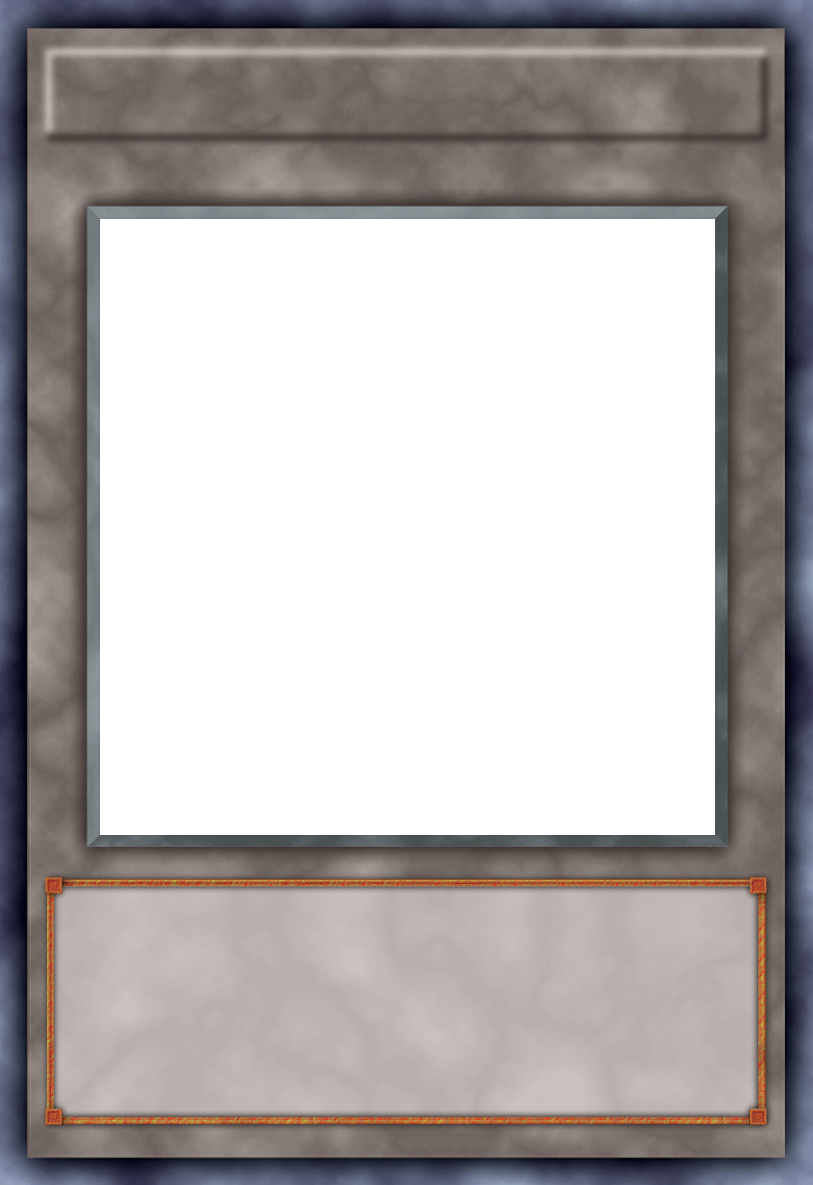
\includegraphics[width=59mm, height=86mm]{card-not-found.png}%
        \llap{%
            \raisebox{78mm}{%
                \resizebox{49mm}{\height}{%
                    \textsc{\detokenize{#1}}%
                }%
            }%
            \hspace{5mm}%
        }%
    }%
}

\begin{document}

    \noindent
    \card{A_D_Changer}
\card{A_D_Changer}
\card{A_D_Changer}
\\[-0.3mm]
\card{Impcantation_Talismandra}
\card{Impcantation_Talismandra}
\card{Impcantation_Bookstone}
\\[-0.3mm]
\card{Impcantation_Bookstone}
\card{Impcantation_Bookstone}
\card{Amano-Iwato}
\\[-0.3mm]
\card{Manju_of_the_Ten_Thousand_Hands}
\card{Manju_of_the_Ten_Thousand_Hands}
\card{Manju_of_the_Ten_Thousand_Hands}
\\[-0.3mm]
\card{Impcantation_Candoll}
\card{Impcantation_Candoll}
\card{Impcantation_Penciplume}
\\[-0.3mm]
\card{Impcantation_Penciplume}
\card{Impcantation_Penciplume}
\card{Shinobaron_Peacock}
\\[-0.3mm]
\card{Shinobaroness_Peacock}
\card{Shinobaroness_Peacock}
\card{Megalith_Phaleg}
\\[-0.3mm]
\card{Megalith_Aratron}
\card{Megalith_Aratron}
\card{Megalith_Aratron}
\\[-0.3mm]
\card{Megalith_Bethor}
\card{Impcantation_Chalislime}
\card{Impcantation_Chalislime}
\\[-0.3mm]
\card{Megalith_Ophiel}
\card{Megalith_Och}
\card{Megalith_Och}
\\[-0.3mm]
\card{Megalith_Och}
\card{Pre-Preparation_of_Rites}
\card{Pre-Preparation_of_Rites}
\\[-0.3mm]
\card{Pre-Preparation_of_Rites}
\card{Extra-Foolish_Burial}
\card{Extra-Foolish_Burial}
\\[-0.3mm]
\card{Pot_of_Avarice}
\card{Preparation_of_Rites}
\card{Preparation_of_Rites}
\\[-0.3mm]
\card{Preparation_of_Rites}
\card{Shinobird's_Calling}
\card{Shinobird's_Calling}
\\[-0.3mm]
\card{Impcantation_Inception}
\card{Impcantation_Inception}
\card{Amorphactor_Pain,_the_Imagination_Dracoverlord}
\\[-0.3mm]
\card{Elder_Entity_N'tss}
\card{Elder_Entity_N'tss}
\card{Elder_Entity_N'tss}
\\[-0.3mm]
\card{Herald_of_the_Arc_Light}
\card{Herald_of_the_Arc_Light}
\card{Herald_of_the_Arc_Light}
\\[-0.3mm]
\card{Gallant_Granite}
\card{Gallant_Granite}
\card{Gallant_Granite}
\\[-0.3mm]


\end{document}


% the contents of cards.tex are generated by a script and should look something like this:

% \card{Mystical_Space_Typhoon}%
% \card{Solemn_Strike}%
% \card{Solemn_Strike}%
% \\[-0.34mm]
% \card{Solemn_Strike}%
% \card{Solemn_Strike}%
% \card{Effect_Veiler}%
% \\[-0.34mm]
% \card{Effect_Veiler}%
% \card{Effect_Veiler}%
% \card{Mystical_Space_Typhoon}%
% \\[-0.34mm]
% \card{Mystical_Space_Typhoon}%
% \card{Mystical_Space_Typhoon}%
% \card{Mystical_Space_Typhoon}%
% \\[-0.34mm]
% \card{Mystical_Space_Typhoon}%
% \card{Solemn_Strike}%
% \card{Solemn_Strike}%
% \\[-0.34mm]
% \card{Effect_Veiler}%
